\documentclass{ctexart}
\usepackage{fontspec, hyperref, wrapfig, graphicx}

\begin{document}
    \title{编译原理(H)报告}
    \author{金孜达、庞茂林、李文睿}
    \maketitle
    \section{项目简介}
    LLVM IR代码优化
    \begin{itemize}
        \item 我们小组的工作是读入 LLVM IR 代码然后使用 LLVM Pass 对代码进行分析以及修改,最终输出优化过的版本,以达到使输出的代码运行更快的目的。
        \item clang 生成的 LLVM IR 在每次 C 语言中调用变量时都会重新执行 load 指令,我们希望去掉这些多余的 load 指令。
    \end{itemize}
    \section{优化原理}
    \subsection{存在的问题}
    \begin{wrapfigure}{r}{.5\textwidth}
        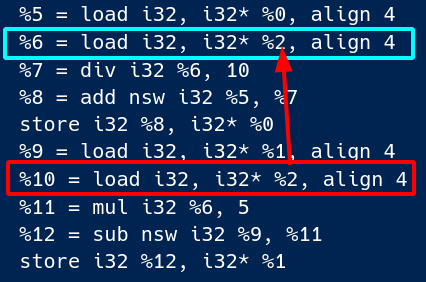
\includegraphics[width=.5\textwidth]{dup_load.png}
        \caption{红色圈出的 load 指令是多余的,可删去}
    \end{wrapfigure}
    以 C 语言为例,在源代码中每个右值在 clang 生成的 LLVM IR 中都会独立执行一次 load 指令,但如果所指代的变量的值在一段时间内没有发生变化,那除了第一次以外,之后的 load 指令都没有必要执行,完全可以复用第一次执行 load 指令的结果,持续到对这个变量进行另一次赋值(在 LLVM IR 中等效为执行一次 store 指令)为止。
    \subsection{优化方法}
    \subsubsection{块内优化}
    对每个块,对每个变量定义一个结构体,包含如下内容:
    \begin{itemize}
        \item load:bool;
        \item loadreg:Value;
        \item alias:vector<Value>;
    \end{itemize}
    该结构体会在该变量被 load 且没有一个对应的结构体时生成,load 值表示该变量已被 load 过,loadreg 表示第一次 load 时接收其值的虚拟寄存器,alias 表示后面几次 load 时接收其值的虚拟寄存器。块内优化时遍历该基本块,该寄存器被 load 时,若 load 为 false,新建立该寄存器对应的 struct,并将 loadreg 赋为接收该 load 返回值的寄存器;若 load 为 true,删掉该 load 语句,并将接收的寄存器放入 alias 中,之后遇到使用 alias 中寄存器的代码,将该寄存器改为 loadreg 中的值。
    \subsection{块间优化}
	块内优化虽已有成效,但不够充分,因为有些变量在未改变值的情况下可以在多个基本块内作为右值,在此情况下这个变量在某些基本块内的 load 指令甚至可以完全删除(仅块内优化是不可能的,因为只要这个变量在这个基本块内至少作过一次右值,那么就会至少有一条 load 指令)。如果在对某个基本块执行块内优化之前,已经知道一些变量在所有到达该基本块路线上都有着一样的 loadreg ,那么就可以将这个 loadreg 作为前提来执行块内优化。当然一开始我们没有任何前提,但是进行迭代,上一次的结果可以计算成为下一次的前提。如此反复直至没有任何改变为止,即完成块间优化。
	
    \subsection{使用的工具}
    我们使用 \href{https://llvm.org/docs/WritingAnLLVMPass.html}{LLVM Pass} 对 LLVM IR 进行分析和优化,通过遍历 bb,计算我们需要的变量以及对代码进行修改。
    \section{遇到的问题}
    一开始的时候我们希望对静态变量进行优化,即如果我们发现该变量对应一个在编译之前即可计算的值,我们会将其值替换为对应的静态常数。
    \begin{itemize}
        \item \%N = \%M \{\%N.s = \%M.s, \%N.val = \%M.val, \%N.p = \%M.p\}
        \item \%N = Uop \%M \{\%N.s = \%M.s, \%N.val = Uop \%M.val, \%N.p = 0\}
        \item \%N = Bop \%A, \%B \{\%N.s = \%A.s \&\& \%B.s \%N.val = \%A.val Bop \%B.val, \%N.p = 0\}
        \item \%N = load i32* \%M \{\%N.s = *\%M.s, \%N.val = *\%M.val, \%N.p = 0\}
        \item store i32 \%M, i32* \%N \{*\%N.s = \%M.s, *\%N.val = \%M.val, \%N.p = 1\}
        \item \%N = alloca i32 * k \{\%N.p = 1, \%N.s = new bool[k], \%N.val = new int[k]\}
        \item \%N = getelementptr \%M, i32 * k \{\%N.p = 1, \%N.s = \%M.s + k, \%N.val = \%M.val + k\}
    \end{itemize}
    但发现在循环中无法使用该方法,因为循环中的值总会变化,而且如果循环在程序开头,那么循环中改变过的变量在后面都无法优化,所以我们先抛弃了这种实现。
    
    之后我们发现可以将编译前未知的值赋为 dirty,接触过 dirty 变量的值也会变为 dirty,然后将程序运行一遍来优化 for 循环中的计算(也可从某方面理解为符号计算)。

    之后发现了可以通过去掉多余的 load 语句来进行优化,这尤其对循环中的优化作用较大,而且在我们的能力范围内能够实现,因此我们选择了该方法。

    其次是使用的工具。

    我们首先想到了使用 lab2-2 中的 assembly\_builder 直接进行优化,之后想到通过 antlr 和 llvm 读取和重新构建代码,最后发现使用 llvm pass 较为简单,而且既可以分析又可以修改,因此选用了它。
    \section{收获和总结}
    在这次编译原理(H)的实验中,我们小组的成员深入讨论了 LLVM IR 优化的方法,通过讨论,改进,抛弃和最后决定,对编译器的优化有了更深的理解。另外我们的组员学习使用了 LLVM Pass,通过不断的尝试调研弄清了如何用 LLVM Pass 来分析、修改 LLVM IR 代码,提高了自身的能力,我们感觉收获了很多。
\end{document}
